\documentclass{beamer}

% Top-aligning columns within a top-aligned frame
% https://tex.stackexchange.com/questions/16447/beamer-top-aligning-columns-within-a-top-aligned-frame
\makeatletter
\newenvironment{myitemize}{%
   \setlength{\topsep}{0pt}
   \setlength{\partopsep}{0pt}
   \renewcommand*{\@listi}{\leftmargin\leftmargini \parsep\z@ \topsep\z@ \itemsep\z@}
   \let\@listI\@listi
   \itemize
}{\enditemize}
\makeatother  

\usepackage[USenglish]{babel}
\usepackage[utf8]{inputenc}
\usepackage{amssymb, amsmath}
\usepackage{bm}
\usepackage{color}
\usepackage{tikz}
\usepackage{url}

\definecolor{links}{HTML}{2A1B81}
\hypersetup{colorlinks,linkcolor=,urlcolor=links}

\usetheme{Boadilla}

\bibliographystyle{apalike}
% make bibliography entries smaller
%\renewcommand\bibfont{\scriptsize}
% Now get rid of all the colours
\setbeamercolor*{bibliography entry title}{fg=black}
\setbeamercolor*{bibliography entry author}{fg=black}
\setbeamercolor*{bibliography entry location}{fg=black}
\setbeamercolor*{bibliography entry note}{fg=black}

\newcommand{\lnorm}[1]{\left\lVert#1\right\rVert^2}
\newcommand{\norm}[1]{\left\lVert#1\right\rVert}

% and kill the abominable icon
\setbeamertemplate{bibliography item}{}

\begin{document}
\title[Mixup (2017)]{Mixup: Beyond Empirical Risk Minimization}  
\author{Radek Bartyzal}
\date{27. 10. 2020} 
\institute{GLAMI AI}

\frame{\titlepage} 

%--------- END Frame 12 -------------
\begin{frame}{Motivation}

\begin{itemize}
\item Empirical Risk Minimization = minimize errors on samples from dataset
\item Data Augmentation = create new samples "around" the existing samples = capture more of the "true" distribution 
\item $\implies$ regularization $\implies$ better generalization
\end{itemize}

\vfill

\textbf{Downsides of classic Data Augmentation:}
\begin{itemize}
\item dataset dependent $\implies$ expert knowledge
\item assumes examples in the vicinity share the same class
\item $\implies$ does not model vicinity relation across examples of different classes
\end{itemize}

\end{frame}

%--------- END Frame 12 -------------
\begin{frame}{Mixup}

\begin{itemize}
\item data agnostic generation of new training samples
\item linear interpolation
\end{itemize}

\begin{figure}[h]
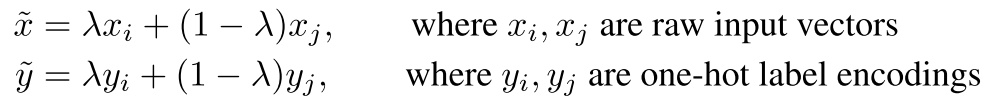
\includegraphics[width=\textwidth]{img/samples}
\caption{Generate new training samples. $\lambda \in [0,1]$}
\end{figure}

\end{frame}
%--------- END Frame 12 -------------
\begin{frame}{Mixup: Easy implementation}

\begin{figure}[h]
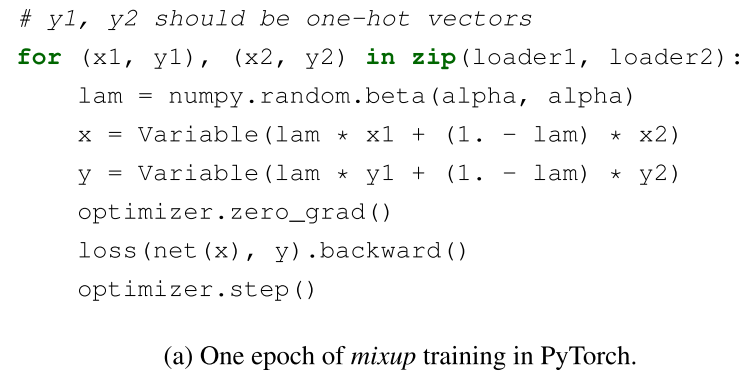
\includegraphics[width=\textwidth]{img/code}

\end{figure}

\end{frame}
%--------- END Frame 12 -------------
\begin{frame}{Mixup: Smoother decision boundary}

\begin{figure}[h]
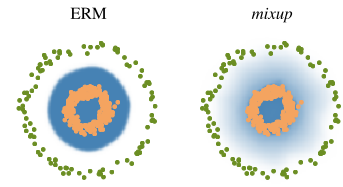
\includegraphics[width=\textwidth]{img/example}
\caption{Effect of mixup $(\alpha = 1)$ on a
toy problem. Green: Class 0. Orange: Class 1. Blue shading indicates $p(y = 1|x)$.}
\end{figure}

\end{frame}
%--------- END Frame 12 -------------
\begin{frame}{Mixup: Vicinal Risk Minimization (VRM)}
VRM approximation of true distribution $P$:

\begin{figure}[h]
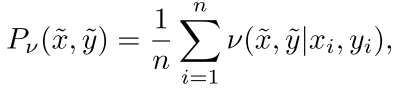
\includegraphics[width=0.5\textwidth]{img/vrm}
\end{figure}

\begin{itemize}
\item $\nu$ is a vicinity distribution that measures the probability of finding the virtual feature-target pair $(\tilde{x}, \tilde{y})$ in the vicinity of the training feature-target pair $(x_i, y_i)$.
\item to train we sample the vicinal distribution to construct a dataset $D_{\nu}$ and minimize the empirical vicinal risk: $R_{\nu}(f)$
\end{itemize}

\begin{figure}[h]
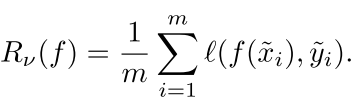
\includegraphics[width=0.5\textwidth]{img/vrl}
\end{figure}

\end{frame}
%--------- END Frame 12 -------------
\begin{frame}{Mixup: Vicinal Risk Minimization (VRM)}
Contribution: Generic vicinal distribution, called mixup:

\begin{figure}[h]
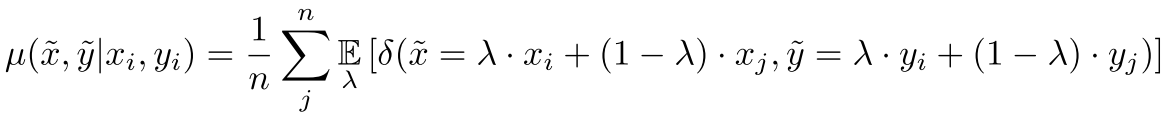
\includegraphics[width=\textwidth]{img/vic_distr}
\end{figure}

\begin{itemize}
\item where $\lambda \sim Beta(\alpha, \alpha)$, for $\alpha \in (0,\inf)$. In a nutshell, sampling from the mixup vicinal distribution produces virtual feature-target vectors:
\end{itemize}

\begin{figure}[h]
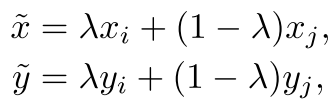
\includegraphics[width=0.5\textwidth]{img/sampling}
\end{figure}

\end{frame}
%--------- END Frame 12 -------------
\begin{frame}{Beta distribution ($\alpha=0.4, \beta=0.4$)}

\begin{figure}[h]
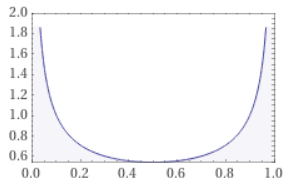
\includegraphics[width=\textwidth]{img/beta}
\end{figure}

\end{frame}

%--------- END Frame 12 -------------
\begin{frame}{Samples generated by Mixup on Two Moons Dataset}

\begin{figure}[h]
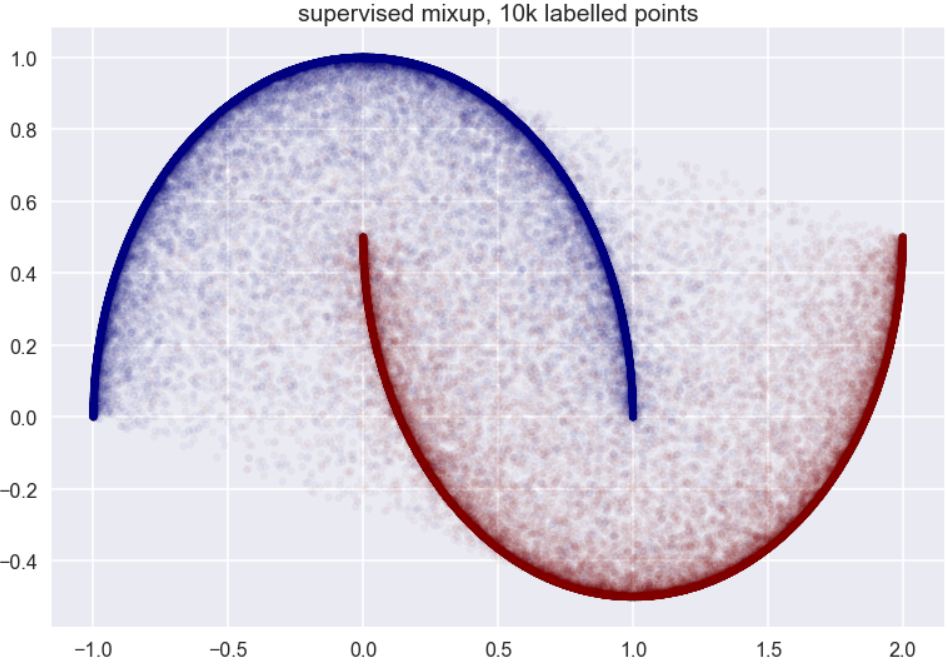
\includegraphics[width=0.9\textwidth]{img/two_moons}
\end{figure}

\end{frame}


%--------- END Frame 12 -------------
\begin{frame}{Mixup: ImageNet results}

\begin{figure}[h]
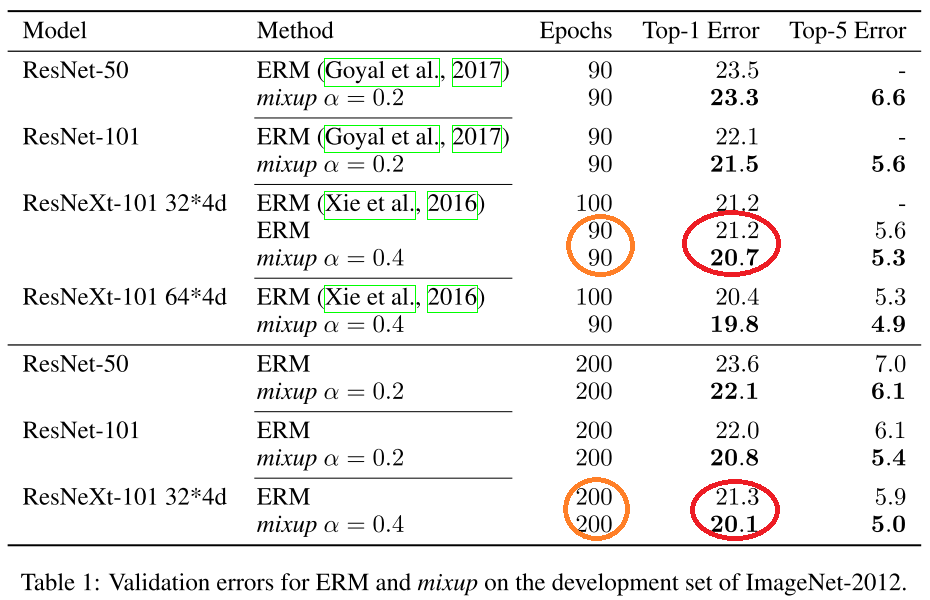
\includegraphics[width=\textwidth]{img/imagenet}
\end{figure}

\end{frame}
%--------- END Frame 12 -------------
\begin{frame}{Mixup: ImageNet results}

\begin{itemize}
\item trained with standard augmentations: scale and aspect ratio distortions, random crops, and horizontal flip
\item $\alpha \in [0.1, 0.4]$ leads to improved performance over ERM
\item large $\alpha \implies$ underfitting 
\item models with higher capacities and/or longer training runs benefit more from mixup
\end{itemize}

\end{frame}
%--------- END Frame 12 -------------
\begin{frame}{Mixup: CIFAR results}

\begin{figure}[h]
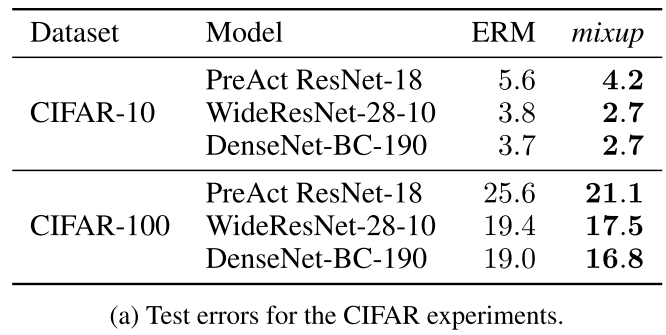
\includegraphics[width=\textwidth]{img/cifar}
\end{figure}

\end{frame}
%--------- END Frame 12 -------------
\begin{frame}{Mixup: Further experiments}

Mixup helps with:
\begin{itemize}
\item speech commands recognition using VGG
\item tabular data: UCI datasets with 2-layer nets trained by Adam
\item robustness against adversarial attacks
\item stabilisation of GAN training
\end{itemize}

\end{frame}

\begin{frame}{Sources}
%--------- END Frame 12 -------------
\begin{thebibliography}{0}

  \bibitem[1]{cit:paper} 1. Zhang, Hongyi, et al. "mixup: Beyond empirical risk minimization." arXiv preprint arXiv:1710.09412 (2017). \url{https://arxiv.org/abs/1710.09412}
  
  \bibitem[2]{cit:fastai} 2. FastAI implementation comments. \url{https://forums.fast.ai/t/mixup-data-augmentation/22764}
  
  \bibitem[3]{cit:inference} 3. INFERENCE blog (two moons analysis). \url{https://www.inference.vc/mixup-data-dependent-data-augmentation/} 
  
\end{thebibliography}

\end{frame}

 
\end{document}
